%% 
%% Copyright 2007-2020 Elsevier Ltd
%% 
%% This file is part of the 'Elsarticle Bundle'.
%% ---------------------------------------------
%% 
%% It may be distributed under the conditions of the LaTeX Project Public
%% License, either version 1.2 of this license or (at your option) any
%% later version.  The latest version of this license is in
%%    http://www.latex-project.org/lppl.txt
%% and version 1.2 or later is part of all distributions of LaTeX
%% version 1999/12/01 or later.
%% 
%% The list of all files belonging to the 'Elsarticle Bundle' is
%% given in the file `manifest.txt'.
%% 
%% Template article for Elsevier's document class `elsarticle'
%% with harvard style bibliographic references

\documentclass[preprint,12pt]{elsarticle}
\usepackage{graphicx}
%% Use the option review to obtain double line spacing
%% \documentclass[preprint,review,12pt]{elsarticle}

%% Use the options 1p,twocolumn; 3p; 3p,twocolumn; 5p; or 5p,twocolumn
%% for a journal layout:
%% \documentclass[final,1p,times]{elsarticle}
%% \documentclass[final,1p,times,twocolumn]{elsarticle}
%% \documentclass[final,3p,times]{elsarticle}
%% \documentclass[final,3p,times,twocolumn]{elsarticle}
%% \documentclass[final,5p,times]{elsarticle}
%% \documentclass[final,5p,times,twocolumn]{elsarticle}

%% For including figures, graphicx.sty has been loaded in
%% elsarticle.cls. If you prefer to use the old commands
\usepackage{epsfig}
\usepackage{longtable}
\usepackage[ruled,vlined]{algorithm2e}
\usepackage{subcaption}
\usepackage{pgfplots}
%% The amssymb package provides various useful mathematical symbols
\usepackage{amssymb}
%% The amsthm package provides extended theorem environments
%% \usepackage{amsthm}

%% The lineno packages adds line numbers. Start line numbering with
%% \begin{linenumbers}, end it with \end{linenumbers}. Or switch it on
%% for the whole article with \linenumbers.
%% \usepackage{lineno}

\journal{Alexandria Engineering Journal}

\begin{document}

\begin{frontmatter}

\title{DecentraliDrone: A Decentralized, Fully Autonomous Drone Delivery System for Reliable, Efficient Transport of Goods}

\author[a]{A Sheik Abdullah\corref{cor1}}
\ead{sheik.abdullah@vit.ac.in}

\author[a]{Abdul Aziz A.B}
\ead{abdulaziz.ahamed2020@vitstudent.ac.in}

\author[a]{S.Geetha\corref{cor1}}
\ead{s.geetha@vit.ac.in}

\cortext[cor1]{Corresponding author(s)}

\address[a]{School of Computer Science and Engineering, Vellore Institute of Technology - Chennai Campus, Chennai 600127, Tamil Nadu, India}


\begin{abstract}
As the world becomes more interconnected and globalized, the demand for efficient and reliable delivery systems is on the rise. To meet this demand, we propose DecentraliDrone, an innovative drone delivery system that utilizes advanced technology to transport goods autonomously and efficiently. Our system is fully decentralized, meaning that it operates without the need for human intervention and relies on a distributed network of drones and devices to function. One of the key features of DecentraliDrone is its autonomy. The system operates without the need for human intervention, enabling it to operate 24/7 and reducing the risk of accidents caused by human error. Additionally, our system is highly scalable, allowing it to adapt to changing demands and expand its delivery capabilities.
There are several challenges that must be addressed in order to fully realize the potential of DecentraliDrone. These include developing robust communication protocols, ensuring the safety and security of the system, and addressing regulatory and legal issues related to autonomous delivery systems.

\end{abstract}\\

%%Graphical abstract
\begin{graphicalabstract}
\includegraphics[width=16cm]{grabs}
\end{graphicalabstract}
%%Research highlights
\begin{highlights}
\item The system ensures faster, accurate deliveries by eliminating human-operated constraints.

\item Real-time routing optimization enhances delivery efficiency, adapting to changing conditions seamlessly.

\item Utilizes Advanced Algorithms for Real-time Danger Detection and Collaborative Decision-making.

\item The system complies with regulations, integrates safety protocols, and prioritizes energy-efficient, environmentally friendly operations.

\item Hybrid drone system that has a greater flight time by using both fuel as well as electric cells.

\end{highlights}

\begin{keyword}
%% keywords here, in the form: keyword \sep keyword
Reinforcement Learning \sep OpenCV \sep Unreal Engine \sep Swarm \sep MetaShape \sep V-SLAM \sep Autonomous System \sep Decentralization
%% PACS codes here, in the form: \PACS code \sep code
\PACS 42.30.Va \sep 07.05.Mh 
%% MSC codes here, in the form: \MSC code \sep code
%% or \MSC[2008] code \sep code (2000 is the default)
\MSC 68T05 \sep 68T40 \sep 68T45 \sep 68U20
\end{keyword}

\end{frontmatter}

\section{Introduction}
Drone delivery systems have the potential to revolutionize the way we transport goods, offering faster and more efficient delivery options compared to traditional methods. However, most existing drone delivery systems rely on human operators to control the drones and make deliveries, which can limit their efficiency and reliability.

To address these challenges, we propose DecentraliDrone, a fully autonomous and decentralized drone delivery system that utilizes advanced technology to ensure reliable and efficient transport of goods. Our system utilizes a network of drones and devices that are able to communicate and coordinate with each other to ensure timely and accurate delivery.

One of the main advantages of DecentraliDrone is its efficiency. By eliminating the need for human operators, our system can make deliveries faster and more accurately than traditional methods. The autonomous drones are equipped with advanced sensors and navigation systems that enable them to navigate their environment and avoid obstacles, ensuring that deliveries are made safely and timely.

In addition to being efficient, DecentraliDrone is also highly reliable. The decentralized nature of our system means that it is able to operate even if individual drones or devices fail. This ensures that deliveries are not disrupted by technical issues and can continue to be made even in the event of a problem.

One of the key challenges in the development of decentralized autonomous drone delivery systems is ensuring the safety of the drones. To address this, DecentraliDrone utilizes a combination of advanced sensors and algorithms to enable the drones to detect and avoid potential collisions. The drones are also equipped with backup systems to ensure that they can continue to operate even if one system fails.

Another challenge in the development of decentralized autonomous drone delivery systems is integrating them into existing logistics and delivery systems. DecentraliDrone addresses this challenge by utilizing a package management module that tracks the location and status of each package and ensures that they are delivered to the correct destination. The system also utilizes a routing module that calculates the most efficient routes for the drones to take in real-time, ensuring that deliveries are made as efficiently as possible.

There are also potential regulatory and environmental challenges to be considered in the development of decentralized autonomous drone delivery systems. DecentraliDrone addresses these issues by following all relevant regulations and utilizing energy-efficient drones and devices that minimize their environmental impact, the decentralized nature of DecentraliDrone allows it to operate in a wide range of environments, including urban, rural, and remote areas. This makes it a versatile delivery solution that can meet the needs of a wide range of users.

We believe this is a promising technology that has the potential to revolutionize the way we transport goods and make a positive impact on society. We look forward to continuing to develop and improve upon this technology in the future.

\section{Components of the System}\\

DecentraliDrones comprises of various essential components, each playing a distinct role in ensuring the successful and efficient delivery of packages. These components are grouped into several key categories, with specific functionalities and tasks assigned to each. The system operates cohesively, combining the efforts of multiple groups to achieve seamless package delivery.

\begin{enumerate}
\item \textbf{Drone Fleet:}
\begin{itemize}
  \item \textbf{Drone Operations Group:}
    \begin{itemize}
      \item Responsible for managing the entire drone fleet.
      \item Monitors drone health and coordinates maintenance activities.
      \item Ensures drones are adequately charged and prepared for deliveries.
    \end{itemize}
  \item \textbf{Drone Routing and Scheduling Group:}
    \begin{itemize}
      \item Develops optimized delivery routes based on package destinations.
      \item Schedules delivery times for maximum efficiency.
      \item Considers factors like weather conditions, traffic, and delivery priorities.
    \end{itemize}
\end{itemize}

\item \textbf{Package Handling:}
\begin{itemize}
  \item \textbf{Loading and Unloading Group:}
    \begin{itemize}
      \item Handles the loading and unloading of packages onto drones.
      \item Ensures secure attachment and proper balancing.
      \item Coordinates with the Drone Operations Group for timely departures.
    \end{itemize}
  \item \textbf{Package Sorting and Categorization Group:}
    \begin{itemize}
      \item Sorts packages based on size, weight, and destination.
      \item Categorizes packages for efficient loading and route planning.
      \item Coordinates with the Drone Routing and Scheduling Group for optimized load distribution.
    \end{itemize}
\end{itemize}

\item \textbf{Navigation and Safety:}
\begin{itemize}
  \item \textbf{Navigation and Guidance Group:}
    \begin{itemize}
      \item Develops and maintains navigation algorithms for drones.
      \item Ensures accurate positioning and obstacle avoidance.
      \item Collaborates with the Drone Routing and Scheduling Group to follow designated routes.
    \end{itemize}
  \item \textbf{Safety and Compliance Group:}
    \begin{itemize}
      \item Monitors regulatory compliance and airspace regulations.
      \item Implements safety protocols to handle emergencies.
      \item Coordinates with local authorities and air traffic control for airspace access.
    \end{itemize}
\end{itemize}

\end{enumerate}\\

These components work together harmoniously to establish a fully functional Drone Delivery System, effectively harnessing the capabilities of autonomous aerial vehicles to transform the delivery industry.

\section{Related Works}

The landscape of Simultaneous Localization and Mapping (SLAM) research has traditionally been dominated by centralized multi-robot systems, prized for their precision but challenged by scalability and adaptability limitations \cite{li2018review}. In response, Swarm SLAM has emerged as a promising alternative, providing decentralized, fault-tolerant mapping, particularly valuable in time-constrained scenarios.

Noteworthy studies have emphasized the significance of decentralized data exchange strategies within Swarm SLAM frameworks \cite{li2018review}. Visual-SLAM (v-SLAM) and Unmanned Aerial Vehicle (UAV) navigation have gained substantial attention, buoyed by the development of bespoke simulators that adeptly navigate challenges associated with physical testing constraints, such as safety restrictions and battery limitations \cite{zhou2018routing}. Furthermore, the fusion of SLAM with sensor data, employing techniques like Extended Kalman Filters, has exhibited prowess in enhancing trajectory estimation \cite{chen2022end}. Low-cost SLAM systems tailored for aerial platforms grappling with limited onboard computing capacity have tactfully leveraged cost-effective sensors, including monocular cameras and altimeters, to calculate precise poses and environmental maps \cite{gupta2022slam}.

Exploration into multi-UAV systems has seen the proposition of cooperative SLAM-based frameworks designed to optimize the flight paths of multiple UAVs while addressing challenges tied to restricted communication bandwidth \cite{munguía2016vslam}. Additionally, avant-garde hybrid drone architectures seamlessly integrating gasoline engines and electric motors have been proffered, showcasing potential benefits such as prolonged flight times and diminished energy consumption—particularly advantageous for applications like package delivery \cite{stolaroff2018energy, jarrah2022flight}.

Incorporating deep learning-based techniques for loop closure detection in SLAM systems has been explored as a promising avenue to augment mapping and localization accuracy \cite{arshad2021loop}. Furthermore, sophisticated path planning methods for autonomous heterogeneous UAVs have been scrutinized, capitalizing on mixed-integer linear programming and clustering-based algorithms to optimize flight paths with precision \cite{chen2022coverage}.

While the presented works collectively contribute to the advancement of SLAM and UAV technologies, certain challenges and lacunae endure. Real-world scenarios may necessitate dynamic obstacle detection, demanding further exploration into path planning techniques \cite{yang2021rrt}. Additionally, the fusion of visual and LiDAR data persists as an ongoing area of research, necessitating the development of tightly coupled LiDAR-vision sensor fusion algorithms \cite{debeunne2020vlidar}.

Concluding the matter, these works furnish a comprehensive overview of the current state of SLAM research, underscoring Swarm SLAM, sensor fusion, and the application of SLAM in UAV systems. The amalgamation of diverse algorithms and technologies manifests as a stride towards surmounting the limitations endemic to centralized systems. However, the persisting challenges—dynamic obstacle detection and sensor fusion—underscore the imperative for sustained exploration and innovation in the field. The proposed method in this study aspires to build upon these foundations, proffering a strategic amalgamation of extant algorithms to furnish a robust and versatile solution for real-world drone missions.

\subsection{Limitations of Existing Works}
The research on Simultaneous Localization and Mapping (SLAM) has predominantly focused on centralized multi-robot systems, yielding precise maps but exhibiting constraints in scalability, adaptability to environmental changes, and resilience in hostile conditions. Swarm SLAM, despite facing technological and financial challenges, offers valuable solutions in scenarios with time or cost constraints and in dynamic environment monitoring \cite{li2018review}.

Related works address various challenges and limitations. Swarm SLAM introduces a decentralized approach, contrasting with the limitations of centralized systems \cite{kegeleirs2021swarm}. The proposed framework leverages existing obstacle avoidance algorithms, namely Proximity Avoidance (PA) \cite{munguía2016vslam}, Dynamic Path Planning (DPP) \cite{lópez2017sensorial}, and Visual-SLAM Integration (VSI) \cite{gupta2022slam}. By amalgamating these algorithms, the framework ensures adaptability, mitigating limitations associated with relying solely on a single predefined algorithm.

The adaptation and enhancement of these algorithms are pivotal. For instance, integrating visual data from a downward-facing camera enhances trajectory estimation and overcomes metric scale recovery issues \cite{chen2022end}. The proposed method draws inspiration from advancements in hybrid multirotor drone architectures, employing gasoline engines for propulsion \cite{jarrah2022flight}.\\\\

Choosing and enhancing the proposed method is rooted in the comprehensive exploration of limitations in existing SLAM and drone delivery systems. The literature review critically analyzes challenges, including scalability, adaptability, environmental monitoring, and energy efficiency. The proposed method addresses these through its decentralized framework, cooperative monitoring, adaptive obstacle avoidance, and algorithmic versatility, enhancing system robustness in real-world scenarios. Integrating existing algorithms provides a nuanced solution, outperforming singular approaches in diverse conditions \cite{stolaroff2018energy, arshad2021loop, chen2022coverage}. This nuanced approach ensures the proposed method's effectiveness, offering a comprehensive solution for real-world drone missions.

\section{Schematics of the Proposed System}
In the context of the system, we have two primary end users, each with distinct roles and responsibilities. 

\subsection{Customer Perspective:}
\begin{enumerate}
\item Place an order within an application that is similar to existing delivery applications.
\item Acquire and place a unique ArUco marker code that is generated in the application at a safe landing spot ie, their roof / balconies etc.
\item Request the delivery.
\item Verify and accept the delivery upon landing.
\end{enumerate}

\subsection{Packing Team Perspective:}
\begin{enumerate}
\item Assemble the items for drone delivery, ensuring they adhere to weight and size specifications compatible with the DecentraliDrone system.
\item Affix the corresponding ArUco marker to the packaged items for seamless recognition during the delivery process.
\item Verify the completeness of the package and ensure all items are properly secured for aerial transportation.
\item If necessary, respond promptly to any alerts indicating potential issues with the delivery, facilitating quick resolution.
\end{enumerate}

\begin{figure}[!htbp]
    \centering
    \includegraphics[width=0.64\linewidth]{methodology.png}
    \caption{DecentraliDrones Methodology Network}
\end{figure}

For the Critic network, the loss function is expressed as:
\begin{equation}
\label{eq:first}
J(\theta_i) = N^{-1}\sum(y - Q_{\theta_i}(S,a))^2
\end{equation}

where:\\
\begin{align*}
&J(\theta_i) \text{ - Critic loss.} \\
&N \text{ - Batch size.} \\
&y \text{ - Target value.} \\
&Q_{\theta_i}(S,a) \text{ - Estimated Q-value.} \\
\end{align*}

For actor networks, a deterministic strategy is used to optimize the parameters, and the loss function is expressed as:
\begin{equation}
\label{eq:second}
{\nabla_\phi}{J(\phi)}=N^{-1}\sum\nabla_{a}Q_{\theta_i}(s,a)|_{a=\Pi_{\phi(s)}}\nabla_{\phi}\Phi_\phi(s)
\end{equation}

where:\\
\begin{align*}
&\nabla_\phi J(\phi) \text{ - Actor loss gradient.} \\
&N \text{ - Batch size.} \\
&Q_{\theta_i}(s,a) \text{ - Estimated Q-value.} \\
&\Pi_\phi(s) \text{ - Deterministic policy.} \\
&\nabla_\phi\Phi_\phi(s) \text{ - Policy gradient.} \\
\end{align*}



The time and space complexity of the TD3 algorithm depend on several factors such as the size of the state and action spaces, the number of layers and neurons in the neural networks, the batch size used for updates, and the length of the training process. 
Overall, the time and space complexity of the TD3 algorithm depend heavily on the size of the neural networks and the batch size used for updates. As these can be adjusted based on the available computational resources, it is difficult to give a general estimate of the complexity of the algorithm. However, it is safe to say that TD3 can be computationally expensive to train, especially for large state and action spaces. \\

\subsection{Basic Architecture Flowchart}\\

\begin{figure}[!htbp]
    \centering
    \includegraphics[width=0.66\linewidth]{arch-enhanced.png}
    \caption{Architecture Flowchart}
\end{figure}

Customers initiate purchase and delivery requests seamlessly through the dedicated app, furnishing essential details such as the destination address and specific order specifications. Each delivery is distinctly identified by a unique ArUco marker code, a pivotal element in facilitating seamless drone operations within the swarm. To ensure the successful delivery process, recipients are tasked with receiving the marker, printing it, and thoughtfully placing it on a suitable, easily accessible surface.

The autonomous journey of the drone unit commences as it is guided by sophisticated path planning algorithms, exemplified by an array of path finding / object avoidance algorithms that are chosen appropriately for the given environmental conditions. This algorithmic intelligence ensures not only obstacle avoidance but also meticulous and effective path planning, guaranteeing a smooth and efficient trajectory toward the designated destination.

Crucially, each delivery is a collaborative effort orchestrated by a pair of drones, each with a specialized role. One drone, entrusted with the payload, adeptly employs V-SLAM technology, contributing to the seamless navigation and delivery execution. Simultaneously, its counterpart provides invaluable visual support, extending the range of vision for the payload-carrying drone and facilitating precise navigation.

Upon reaching the destination vicinity, the drone pair meticulously initiates the search for the pre-designated ArUco marker, employing the sophisticated openCV component for efficient marker detection. The marker, once located and verified, acts as the authentication for the completion of the delivery. This successful accomplishment triggers prompt updates on the app interface and the central logger, ensuring transparency and real-time information dissemination.

However, in cases where the ArUco marker is not promptly found or is situated in an unsuitable environment, the drone takes a proactive stance. It raises a request within the app interface, signaling the need for recipient intervention. The recipient, in turn, must respond promptly to rectify the marker's placement within a defined timeframe. This timely interaction is crucial, as it determines the acceptance or redirection of the raised request. Failure on the recipient's part to respond within the stipulated time prompts the drone unit to gracefully initiate its return journey to the dispatch unit, conscientiously logging the scenario as an incomplete delivery. This robust and adaptive process ensures the efficiency and reliability of the entire delivery mechanism.

\subsection{Swarm Schematics}
\begin{figure}[!htbp]
    \centering
    \includegraphics[width=8.5cm, height=7cm]{images/Decentralized_Structure.png}
    \caption{Decentralized Swarm Structure of Drone Network}
\end{figure}

This schematic explains the basic workings behind the communications involved among the swarm of drones that are deployed, being a decentralised system, they check in on each other for the delivery states and carry out the delivery screening process where they travel around the delivery point and drop the packages where and when required. The drones also keep track of the individual check ins so that when one of the drones faults to an unfortunate circumstance, the system balances itself by sending in a replacement by peer communication via the group check in feature.\\

\begin{figure}[!htbp]
    \centering
    \includegraphics[width=8cm, height=8cm]{images/communication_schematics.png}
    \caption{Drone Activity Diagram}
\end{figure}

The following diagram gives a sharp overview of the communication that occurs among the drones to make successful deliveries, being in a decentralised system, the drones are their own controller entity as a whole system, the success of the system is considered as a group effort rather than a singular entity’s success, keeping this in mind, the drones communicate with each other to make sure that the deliveries are made. The communication is done through cellular towers present across the region where the drones are deployed for delivering the goods.\\

\subsection{Functional Quad-rotor Schematics}\\

\begin{figure}[!htbp]
    \centering
    \includegraphics[width=9.5cm, height=8.5cm]{images/quad-rotor_schematics.png}
    \caption{Single Drone Schematic Diagram}
\end{figure}

The following diagram explains the functioning of a singular entity from the system of swarm. Each quad-rotor entity has its own guidance system that is line of sight based, acting upon which the motors and propellers are instructed to take the ascend or descend of the drone, it uses computer vision algorithms to perform obstacle detection and avoidance, the guidance system gives the appropriate trajectory for the drone to take in order to make a successful delivery happen in accordance to the environmental factors that are laid upon in its path. The Guidance system takes the inputs from the navigation system and performs the appropriate logical decisions to map out the path for the drone.\\

\subsection{Takeoff and Landing for VTOL Schematics}\\
The illustrated diagram provides a comprehensive depiction of the intricate takeoff and landing sequence of the drone. Notably, the drone is strategically designed to land precisely on specified markers during each delivery. This precision landing mechanism is a fundamental component of the overall system, ensuring that the drone consistently lands and takes off at predetermined locations.

The underlying technology facilitating this process is a Vertical Takeoff and Landing (VTOL) system, which incorporates sophisticated altitude and position control. This system plays a pivotal role in orchestrating the drone's movements, allowing it to navigate with precision and accuracy during both takeoff and landing phases.

To further enhance operational efficiency and safety, the drone is equipped with fall detection systems. These systems serve a crucial function by promptly detecting any instances of unplanned descents or falls. In the event of such incidents, the fall detection systems generate alerts, notifying other drones within the swarm.\\\\

\begin{figure}[!htbp]
    \centering
    \includegraphics[width=10cm, height=9.5cm]{images/takeoff_landing.png}
    \caption{Takeoff and Landing Pre-flight Schematics for Single Drone}
\end{figure}

These alerts serve a dual purpose – not only do they signal the need for immediate maintenance for the affected drone, but they also communicate the status of an incomplete delivery. Subsequently, neighboring drones in the vicinity can make informed decisions about whether to take charge of the pending delivery or provide support for maintenance activities.

\begin{table}[htbp]
  \centering
  \caption{Multicopter Specifications}
  \begin{tabular}{lcccc}
    \toprule
    Model & Airframe Mass (kg) & Total (kg) & Flight Time (min) & Takeoff (kg) \\
    \midrule
    DJI Matrice 600 & 5.96 & 9.5 & 32 & 15.1 \\
    DJI M200 & 2.76 & 3.80 & 27 & 6.1 \\
    Kitty Hawk & 4.08 & 9.15 & 30 & 18.6 \\
    \bottomrule
  \end{tabular}
\end{table}\\

\begin{table}[htbp]
  \centering
  \caption{HES Aerostak Fuel Cell Specifications}
  \begin{tabular}{lccccc}
    \toprule
    Power (W) & Mass (kg) & L/min & Pressure (bar) & Equivalent Volume (L) & Time (s) \\
    \midrule
    200 & 2.06 & 2.8 & 0.5 & 1200 & 25714 \\
    500 & 2.90 & 6.5 & 0.5 & 1200 & 11077 \\
    1000 & 3.75 & 14 & 0.55 & 1091 & 4675 \\
    \bottomrule
  \end{tabular}
\end{table}\\


The energy efficiency of a drone can be calculated as the ratio of useful work (such as lifting a payload or performing a task) to the energy input (typically from the battery):
\begin{equation}
\text{Energy Efficiency (\%)} = \frac{\text{Useful Work}}{\text{Energy Input}} \times 100
\end{equation}

The flight time of a drone can be estimated using the following equation:
\begin{equation}
\text{Flight Time (minutes)} = \frac{\text{Battery Capacity (Wh)}}{\text{Power Consumption (W)}}
\end{equation}
Where:
Battery Capacity (Wh) is the capacity of the drone's battery in watt-hours.
Power Consumption (W) is the average power consumption of the drone during flight.
It's important to note that power consumption varies based on factors such as drone weight, motor efficiency, aerodynamics, and flight conditions.

The endurance of a drone refers to how long it can stay in the air under specific conditions. It can be calculated using a similar equation to flight time:
\begin{equation}
\text{Endurance (minutes)} = \frac{\text{Battery Capacity (Wh)}}{\text{Power Consumption (W)}}
\end{equation}
The endurance equation is particularly useful when optimizing drones for specific missions or tasks where extended flight time is essential.

The energy consumption rate of a drone can be expressed as:
\begin{equation}
\text{Consumption Rate (Wh/min)} = \frac{\text{Battery Capacity (Wh)}}{\text{Flight Time (min)}}
\end{equation}
This equation helps you understand how quickly a drone consumes its battery energy during flight.

Table 2  underscores the fuel cell's efficiency by revealing its ability to deliver significant power output (200 W to 1000 W) while consuming relatively small amounts of hydrogen (2.8 L/min to 14 L/min). These specifications demonstrate its suitability for applications where both power and fuel efficiency are crucial, making it an environmentally friendly and cost-effective choice for energy generation.


\subsection{CAD Model Description}

\begin{enumerate}
    \item \textbf{Drone Configuration:} The hybrid drone is designed in the Quad(X) Configuration, which provides stability and maneuverability.

    \begin{figure}[!htbp]
    \centering
    \includegraphics[width=8cm, height=4cm]{images/X_config.png}
    \caption{Drone in X Config}
    \end{figure}

    \item \textbf{Hybrid Power-Based Design:} The drone features a hybrid power-based design, combining four electric motors with two petrol engines to optimize energy consumption and flight time.\\

    \begin{figure}[!htbp]
    \centering
    \vspace{-0.5cm}
    \includegraphics[width=8cm, height=4cm]{images/config2.png}
    \caption{Hybrid Model}
    \end{figure}

    \item \textbf{Protective Dome:} A synthetic dome covers the brain of the drone, housing sensitive sensors, flight controllers, and microcontrollers. It safeguards critical components.\\

    \begin{figure}[!htbp]
    \centering
    \vspace{-0.5cm}
    \includegraphics[width=6cm, height=3cm]{images/dome.png}
    \caption{Protective Dome of Drone}
    \end{figure}

    \item \textbf{Hybrid Power Source:} The drone is equipped with a fuel tank serving as a hybrid power source, ensuring extended flight duration.\\

    \begin{figure}[!htbp]
    \centering
    \includegraphics[width=8cm, height=4cm]{images/fuel_tank.png}
    \caption{Side View of Fuel Tank}
    \end{figure}
    
    \begin{figure}[!htbp]
    \centering
    \includegraphics[width=8cm, height=4cm]{images/fuel_tank2.png}
    \caption{Bottom View of Fuel Tank}
    \end{figure}

    \item \textbf{Manipulator Component:} The drone is equipped with tentacular manipulators designed to handle associated payloads effectively.\\

    \begin{figure}[!htbp]
    \centering

    \includegraphics[width=8cm, height=4cm]{images/manipulator.png}
    \caption{Drone Tentacular Manipulators}
    \end{figure}
\end{enumerate}

\subsection{Proposed Framework and Architecture}
The drone's architecture follows a decentralized approach, enabling it to work autonomously and collaboratively within a swarm. The framework incorporates various communication protocols, algorithms for path planning, and optimization techniques.

\subsubsection{Protocols}
Communication among the drone swarm is facilitated through custom protocols designed to ensure seamless coordination.

\subsubsection{Path Planning and Optimization Algorithms}
The drone employs sophisticated path planning algorithms, such as TD3, for obstacle avoidance, course correction, and efficient navigation. Optimization algorithms are integrated to enhance energy efficiency and route selection.

\subsection{Computer Vision-Based Components}
The drone leverages computer vision algorithms for tasks like object detection, marker recognition, and visual navigation. This includes Visual SLAM and other relevant techniques.

\subsection{CAD Design and Specifications}
The CAD design incorporates specific dimensions, materials, and structural details. Specifications include payload capacity, flight range, and more.


\begin{table}[!htbp]
\centering
\caption{Specifications and Values}
\begin{tabular}{|l|l|}
\hline
Specification       & Value             \\
\hline
Payload Capacity    & 20 kg             \\
Flight Range        & 200 km            \\
Battery Capacity    & 25,000 mAh        \\
Maximum Speed       & 100 km/h          \\
Fuel Tank Capacity   & 10 liters         \\
\hline
\end{tabular}
\end{table}

\subsection{Formulas and Equations}

\begin{equation}
\text{Energy Consumption} = \frac{\text{Fuel Consumed}}{\text{Flight Distance}}
\end{equation}
For calculating the energy consumption of the hybrid drone by dividing the amount of fuel consumed by the distance traveled during the flight.

\begin{equation}
\text{Optimization Objective} = \sum_{i=1}^{n} C_i x_i
\end{equation}
To represent an optimization objective where \(\sum_{i=1}^{n}\) indicates the sum of all \(n\) optimization factors (e.g., energy efficiency, path length) weighted by their respective coefficients \(C_i\).

\begin{equation}
\text{Path Length} = \int_{t_0}^{t_1} \sqrt{(dx/dt)^2 + (dy/dt)^2} dt
\end{equation}
Was used to compute the path length during a drone's flight by integrating the Euclidean distance over time, where \(dx/dt\) and \(dy/dt\) are the rate of change of the drone's position in the x and y directions.

\begin{equation}
\text{Marker Recognition Accuracy} = \frac{\text{Correct Matches}}{\text{Total Matches}}
\end{equation}
For measuring the marker recognition accuracy, which is the ratio of correctly recognized markers to the total number of matched markers.

\begin{equation}
\text{Fuel Efficiency} = \frac{\text{Flight Distance}}{\text{Fuel Consumed}}
\end{equation}
The formula calculates the fuel efficiency of the drone by dividing the flight distance by the amount of fuel consumed.

\begin{equation}
\text{Time to Destination} = \frac{\text{Distance}}{\text{Speed}}
\end{equation}
Computes the estimated time required to reach the destination based on the distance to be covered and the drone's speed.

\begin{equation}
\text{Takeoff Thrust} = \text{Weight} + \text{Lift Force}
\end{equation}
Takeoff thrust is determined by adding the weight of the drone to the required lift force to overcome gravity.

\begin{equation}
\text{Landing Approach Angle} = \tan^{-1}\left(\frac{\text{Vertical Descent Rate}}{\text{Horizontal Approach Speed}}\right)
\end{equation}
Calculates the landing approach angle, which is the angle at which the drone descends during the landing phase.

\begin{equation}
\text{Aerodynamic Lift} = \frac{1}{2} \times \text{Air Density} \times \text{Aerodynamic Coefficient} \times \text{Wing Area} \times \text{Velocity}^2
\end{equation}
The aerodynamic lift force acting on the drone's wings, considering factors such as air density, aerodynamic coefficient, wing area, and velocity.

\begin{equation}
\text{Drag Force} = \frac{1}{2} \times \text{Air Density} \times \text{Drag Coefficient} \times \text{Frontal Area} \times \text{Velocity}^2
\end{equation}
The drag force experienced by the drone, considering air density, drag coefficient, frontal area, and velocity.




\section{Result Comparison of Existing and Our System}
\textit{A Brief Overview of Parameters}\\


\subsubsection{Best Y}\\
The \textit{"best Y vs episode" }graph shows the maximum reward achieved by the agent in each episode during training. The graph is useful for evaluating the overall performance of the agent during training. The graph shows a steady increase in the maximum reward achieved over the course of training, indicating that the agent is improving its performance.\\

In the early episodes of training, the maximum reward achieved may be low but as it progresses, the maximum reward achieved should increase as the agent becomes more skilled at selecting actions that lead to higher rewards.
The shape of the graph can vary depending on the specific environment and hyperparameters used for training. However, in general, it should show a positive trend over time. If the graph shows a plateau or a decline in the maximum reward achieved, it may indicate a problem with the training process or the environment. \\

\subsubsection{Actor loss}\\
The graph of \textit{“Actor loss vs episodes” } shows how the loss of the actor changing over the course of training. The actor loss is a measure of how well the actor can select actions that lead to higher rewards. Typically, the actor loss decreases over the course of training as the actor becomes better at selecting actions.\\
In the early episodes of training, the actor loss is high as the actor explores the environment and tries out different actions. As training progresses, the actor becomes more confident in its actions, and the loss decreases. If the actor loss does not decrease over the course of training, it indicates a problem with the training process or the environment itself. In such cases, it may be necessary to adjust the hyperparameters or try different training techniques to improve performance.\\

\subsubsection{Critic loss}\\
The \textit{critic loss vs episode graph} shows the loss of the critic changing over the course of training. The critic loss is a measure of how well the critic can estimate the value of the current state. Critic loss decreases over the course of training as the critic becomes better at estimating the state value. 

In the early episodes of training, the critic loss may be high but as it progresses, the critic becomes more confident in its estimates, and the loss decreases. If the critic loss does not decrease over the course of training, it indicates a problem with the training process or the environment itself. In such cases, it may be necessary to adjust the hyperparameters or try different training techniques to improve performance.\\

\subsubsection{Level}\\
The \textit{level vs episode graph} shows how the agent's performance on different levels or stages of the environment changes over the course of training. This graph is particularly useful when training the agent on environments with different levels or stages, such as video games with multiple levels. Each point on the graph represents the agent's performance on a particular level or stage during a specific episode of the training process. The performance can be measured by different metrics such as cumulative reward, time taken to complete the level, or accuracy.\\
This graph can provide valuable insights into how the agent is progressing through the levels or stages of the environment. Ideally, the graph should show a steady increase in performance on each level over the course of training. If the agent is struggling on certain levels or stages, this can be identified by a plateau or a decline in performance on the corresponding levels.\\
The shape of the graph can vary depending on the specific environment and hyperparameters used for training. In general, the graph should show a positive trend in performance over time. However, there may be some variability in performance on individual levels or stages, which can be influenced by factors such as the level's difficulty, the randomness of the environment, or the agent's exploration strategy.\\

\subsubsection{P max}\\
The \textit{"p max vs episode"} graph shows how the maximum probability of the actions selected by the actor changes over the course of training. The maximum probability (p max) is the highest probability assigned by the actor to any action in each state.\\
Ideally, the graph should show a decreasing trend in p max over the course of training, indicating that the actor is becoming more confident in its actions and selecting a wider range of actions.\\
In the early episodes of training, the p max may be high but as it progresses, the actor becomes more confident in its actions, and the p max decreases. This is a desirable outcome as a high p max indicates that the actor is not exploring enough and is potentially stuck in a suboptimal policy.\\
If the p max does not decrease over the course of training, it may indicate a problem with the training process or the environment itself. In such cases, it may be necessary to adjust the hyperparameters or try different training techniques to improve performance.\\

\subsubsection{Score}\\
A \textit{"score vs episode graph"} is a common way to visualize performance. As the agent learns and improves its policy and value functions through training, one expects to see an upward trend in the score vs episode graph. In the beginning, the agent's performance may be poor, and the score may fluctuate wildly. As the agent learns, however, the score should become more consistent and gradually increase.\\

\subsubsection{Step}\\
A \textit{"step vs episode graph"} is another way to visualize the performance of a reinforcement learning algorithm. The x-axis represents the episodes or iterations of the algorithm, and the y-axis represents the total number of steps taken by the agent in each episode.\\
Each step represents an interaction between the agent and the environment, where the agent selects an action based on its current policy, receives a reward from the environment, and transitions to a new state. The goal of the agent is to learn a policy that maximizes the cumulative reward over many steps.\\

\subsubsection{Action}\\
The \textit{"Average action vs episode" graph} shows how the average action taken by the agent changes over time as it interacts with the environment. The average action is typically calculated by taking the mean of the actions taken by the agent across a given episode or time step. It can provide insights into how the agent is exploring the environment and making decisions.\\
If the average action remains constant or fluctuates significantly over time, it may indicate that the agent is not effectively exploring the environment or is having difficulty learning an optimal policy.
On the other hand, if the average action decreases over time, it may indicate that the agent is becoming more conservative in its decision-making and focusing on exploiting known high-reward actions. This behavior may be desirable in certain scenarios, such as when the environment is relatively stable and the agent has learned a good policy.\\
Alternatively, if the average action increases over time, it may indicate that the agent is becoming more exploratory and trying out new actions in the environment. This behavior may be desirable in scenarios where the agent needs to discover new high-reward actions or adapt to changes in the environment.\\

\subsubsection{Q value}\\
\textit{Q-values} signify the expected reward for an action in a state, pivotal in RL algorithms like Q-Learning. The graph plots episodes (x-axis) against the average Q-value of the learned policy (y-axis), demonstrating the agent's learning progress. A steady increase typically reflects improved understanding of the environment. The graph's shape provides insights: a swift early rise suggests quick learning, while a slower ascent may indicate the need for more training or a different algorithm.

\subsubsection{Average Velocity}\\
The \textit{average velocity versus episodes graph} is a way of visualizing the learning progress of an RL algorithm in a control task where the goal is to control the velocity of an agent. \\

\subsection{Recurrent Advantage Actor Critic Agent for Airsim }\\

The Advantage Actor-Critic (A2C) algorithm is a reinforcement learning algorithm that combines two approaches: policy gradient and value function estimation. It is commonly used for solving continuous action space environments, where the optimal action cannot be easily determined by the agent. It consists of 2 components: an actor and a critic. The actor is responsible for selecting actions based on the current state, critic evaluates the value of the current state. They work together to improve the agent's performance in the given environment.\\
The actor takes current states as the inputs and outputs a probability distribution over the possible actions. The critic takes the current states as input and outputs an estimate of the state's value. The value function estimate represents expected cumulative reward the agent receives from that state onwards.\\
\begin{algorithm}[!htbp]
\caption{Advantage Actor-Critic (RA2C) Algorithm}
\begin{algorithmic}
    \STATE Initialize actor $\pi(a|s,\theta)$ and critic $V(s,\omega)$ with parameters $\theta$ and $\omega$\\
    \STATE Initialize environment, hyperparameters, and training parameters\\
    \FOR{each episode}\\
        \STATE Initialize state $s$\\
        \FOR{each time step}\\
            \STATE Select action $a \sim \pi(\cdot|s,\theta)$ using the actor\\
            \STATE Execute action $a$, observe reward $r$ and next state $s'$\\
            \STATE Calculate advantage $A(s,a)$ using critic's estimate\\
            \STATE Update actor's policy using policy gradient:\\
            \STATE \quad $\theta \leftarrow \theta + \alpha \nabla_\theta \log \pi(a|s,\theta) \cdot A(s,a)$\\
            \STATE Update critic's value function using temporal difference error:\\
            \STATE \quad $\omega \leftarrow \omega + \beta \nabla_\omega [V(s,\omega) - (r + \gamma V(s',\omega))]^2$\\
            \STATE $s \leftarrow s'$\\
        \ENDFOR\\
    \ENDFOR\\
\end{algorithmic}
\end{algorithm}

\subsubsection{Best Y}\\
An increase in the Best Y graph typically indicates the agent's learning and performance improvement over time. It suggests that the agent is discovering better policies for interacting with the environment, resulting in higher rewards or enhanced performance.\\
\begin{figure}[!htbp]
    \centering
    \includegraphics[width=9.5cm, height=4cm]{./images/Best Y.png}
    \caption{Best Y graph for RA2C}
\end{figure}


\subsubsection{Actor loss}\\
Actor loss graph remains the same over time, it suggests that the actor network has converged to a local minimum, and is no longer improving its policy. This can happen when the agent has reached a plateau in its learning, and has found a sub-optimal policy that is "good enough" for the current task. In this case, further updates to the actor network may not result in significant improvements in performance.\\

\begin{figure}[!htbp]
    \centering
    \includegraphics[width=9.5cm, height=4cm]{./images/Actor loss.png}
    \caption{Actor loss graph for RA2C}
\end{figure}

\textbf{Critic loss}\\
The Critic Loss graph shows a decreasing trend with occasional fluctuations over time. This indicates that the agent is learning and improving its value function. However, it may still be exploring different policies or facing some degree of uncertainty in the environment.\\
\begin{figure}[!htbp]
    \centering
    \includegraphics[width=9.5cm, height=4cm]{./images/Critic loss.png}
    \caption{Critic loss graph for RA2C}

\end{figure}

\subsubsection{P max}\\
The Pmax graph initially ascends, signaling the agent's refinement of its policy and increased confidence in action selection. Following this, a plateau emerges, indicating that the agent has attained a reasonable level of confidence in its policy. Consequently, the agent curtails further exploration, as additional efforts may yield only marginal improvements in the policy.\\

\begin{figure}[!htbp]
    \centering
    \includegraphics[width=9.5cm, height=4cm]{./images/P max.png}
    \caption{P max graph for RA2C}
\end{figure}
\vspace{-0.5cm}
\subsubsection{Level}\\
The Level graph shows a consistent increase over time, indicating that the agent is steadily improving its performance on the task at hand.\\
\begin{figure}[!htbp]
    \centering
    \includegraphics[width=10.5cm, height=6cm]{./images/Level.png}
    \caption{Level graph for RA2C}
\end{figure}
\vspace{-0.5cm}
\subsubsection{Score}\\
The Score graph exhibits a consistent increase over time, indicating that the agent is steadily enhancing its performance on the task at hand.\\
\begin{figure}[!htbp]
    \centering
    \includegraphics[width=9.5cm, height=4cm]{./images/Score.png}
    \caption{Score graph for RA2C}
\end{figure}

\subsubsection{Step}\\
The Step graph displays fluctuations over time, indicating that the agent might be encountering challenges or instability in learning the task. Possible reasons include overfitting, suboptimal policy discovery, or instability.\\
\begin{figure}[!htbp]
    \centering
    \includegraphics[width=9.5cm, height=4cm]{./images/Step.png}
    \caption{Step graph for RA2C}
\end{figure}
 
\\

\subsection{Recurrent Deep Deterministic Policy Gradient}\\
The Recurrent Deep Deterministic Policy Gradient (RDPG) algorithm is a type of reinforcement learning algorithm used to train deep neural networks to learn optimal policies for sequential decision-making problems. RDPG is an extension of the Deep Deterministic Policy Gradient (DDPG) algorithm, which itself is a variant of the Q-learning algorithms.\\

It optimizes a policy network and a value network simultaneously. The policy network takes the current state of the environment as input and outputs an action to be taken. The value network takes the current state and the action chosen by the policy network as input and outputs an estimate of the expected return from that state-action pair.\\

It extends DDPG by introducing a recurrent neural network (RNN) into the policy network. The RNN allows the policy network to maintain a memory of past states and actions, which can be used to inform future decisions. This is particularly useful in tasks where the optimal action depends on a sequence of past actions and observations.\\

The policy network is also trained to maximize the expected return over a sequence of actions. The value network is trained to minimize the difference between its estimate of the expected return and the actual return received after taking a sequence of actions. Both networks are updated using backpropagation through time (BPTT), which is a variant of backpropagation that allows gradients to be computed over a sequence of inputs.\\
\begin{algorithm}\\
\caption{Recurrent Deep Deterministic Policy Gradient (RDDPG) Algorithm}
\begin{algorithmic}
    \STATE Initialize policy network $\pi_{\theta}$ and value network $V_{\phi}$ with parameters $\theta$ and $\phi$\\
    \STATE Initialize environment, hyperparameters, and training parameters\\
    \FOR{each episode}\\
        \STATE Initialize recurrent state $h_0$\\
        \STATE Initialize state $s_0$\\
        \FOR{each time step}\\
            \STATE Sample action $a_t \sim \pi_{\theta}(s_t, h_t)$ from the policy network\\
            \STATE Execute action $a_t$, observe reward $r_t$, and new state $s_{t+1}$\\
            \STATE Update recurrent state $h_{t+1}$ using the RNN dynamics\\
            \STATE Calculate the advantage estimate $A_t$\\
            \STATE Update policy network and value network using backpropagation through time (BPTT):\\
            \STATE \quad Policy network update: $\theta \leftarrow \theta + \alpha \nabla_\theta\\ J(\theta)$\\
            \STATE \quad Value network update: $\phi \leftarrow \phi + \beta \nabla_\phi\\ \left(\frac{1}{2}(V_\phi(s_t, h_t) - (r_t + \gamma V_\phi(s_{t+1}, h_{t+1})))^2\right)$\\
            \STATE $s_t \leftarrow s_{t+1}$, $h_t \leftarrow h_{t+1}$\\
        \ENDFOR\\
    \ENDFOR\\
\end{algorithmic}
\end{algorithm}

\subsubsection{Actor Loss}\\
The \textit{Actor loss} graph initially rises, indicating the agent's exploration of various policies. Subsequently, it decreases as the agent refines its strategy and converges towards a better solution. The initial increase may stem from the exploration phase, testing different policies, possibly leading to suboptimal choices. With increased experience and policy updates based on rewards, the actor loss diminishes as the agent converges to an improved solution.
\begin{figure}[!htbp]
    \centering
    \includegraphics[width=9.5cm, height=4cm]{./images/Actor loss.png}
    \caption{Actor loss graph for RDDPG}
\end{figure}\\

\subsubsection{Average Action (Noise)}\\
\textit{Avg Action (noise)} graph fluctuates over time, suggesting that the agent is experiencing some level of instability or variability in its exploration behavior.
\begin{figure}[!htbp]
    \centering
    \includegraphics[width=9.5cm, height=4cm]{./images/Avg Action (noise).png}
    \caption{Average action noise graph for RDDPG}
\end{figure}

\subsubsection{Average Q}\\
\textit{Average Q} graph increases over time, suggesting that the agent is improving its estimates of the optimal state-action value function and making better decisions.
\begin{figure}[!htbp]
    \centering
    \includegraphics[width=9.5cm, height=4cm]{./images/Avg Q.png}
    \caption{Average Q graph for RDDPG}
\end{figure}

\subsubsection{Average velocity}\\
\textit{Average velocity} graph increases initially and then plateaus over time, suggesting that the agent is improving its ability to move efficiently through the environment but has reached a limit in its performance. It may be necessary to adjust the agent's training parameters or explore new techniques to continue improving its performance. Alternatively, the plateau in average velocity may be due to the environment itself.
\begin{figure}[!htbp]
    \centering
    \includegraphics[width=9.5cm, height=4cm]{./images/Avg velocity.png}
    \caption{Average velocity graph for RDDPG}
\end{figure}

\subsubsection{Best Y}\\
\textit{Best Y} When this graph increases, it typically means that the agent is learning and improving its performance over time. Specifically, it suggests that the agent is finding better policies for interacting with the environment, resulting in higher rewards or better performance.
\begin{figure}[!htbp]
    \centering
    \includegraphics[width=9.5cm, height=4cm]{./images/Best Y.png}
    \caption{Best Y graph for RDDPG}
\end{figure}

\subsubsection{Critic Loss}\\
\textit{Critic Loss} graph increases over time, suggesting that the agent is not learning effectively and is not improving its value function as it may have a high learning rate, architecture may not be well-suited, or the rewards may be delayed.
\begin{figure}[!htbp]
    \centering
    \includegraphics[width=10.5cm, height=6cm]{./images/Critic Loss.png}
    \caption{Critic loss graph for RDDPG}
\end{figure}

\subsubsection{Level}\\
\textit{Level} graph increases over time, suggesting that the agent is improving its performance on the task at hand.
\begin{figure}[!htbp]
    \centering
    \includegraphics[width=10.5cm, height=6cm]{./images/Level.png}
    \caption{Level graph for RDDPG}
\end{figure}

\subsubsection{Score}\\
\textit{Score} graph increases over time, suggesting that the agent is improving its performance on the task at hand.
\begin{figure}[!htbp]
    \centering
    \includegraphics[width=10.5cm, height=6cm]{./images/Score.png}
    \caption{Score graph for RDDPG}
\end{figure}

\subsubsection{Step}\\
\textit{Step} graph fluctuates over time, suggesting that the agent is experiencing some level of instability in its learning process.
\begin{figure}[!htbp]
    \centering
    \includegraphics[width=10.5cm, height=6cm]{./images/Step.png}
    \caption{Step graph for RDDPG}
\end{figure}


\subsection{Recurrent Deep Deterministic Policy Gradient with PER}
Recurrent Deep Deterministic Policy Gradient with Prioritized Experience Replay (RDPG-PER) holds significant promise in drone applications, where autonomous decision-making in complex and dynamic environments is paramount.\\

By incorporating a recurrent neural network (RNN), RDPG-PER enables drones to make informed, sequential decisions that consider past observations and actions, vital for tasks such as mapping, exploration, and surveillance. The integration of Prioritized Experience Replay (PER) enhances learning by prioritizing experiences, making it particularly valuable for drones encountering critical or rare events during training. \\
This combination of recurrent architectures, prioritized learning, and adaptability equips drones with efficient and stable policy improvement, allowing them to navigate diverse and non-stationary environments effectively. \\

Additionally, RDPG-PER enhances long-term planning capabilities, crucial in applications like search and rescue missions, making use of the priority experience replay to get a grasp of what went wrong and avoid that, preventing the wastage of training hours that went into training the model. In drone applications, particularly in mapping and exploration tasks, the ability to remember previously visited locations and adapt actions based on prior mapping data is crucial. The RNN in RDPG-PER enables drones to maintain a memory of the environment, facilitating efficient exploration and mapping over time. RDPG-PER's recurrent architecture, combined with prioritized learning, equips drones with the ability to plan and execute actions that maximize mission success over extended periods. \\

\begin{algorithm}[!htbp]
\caption{Recurrent Deep Deterministic Policy Gradient with Prioritized Experience Replay (RDPG-PER) Algorithm}
\begin{algorithmic}
    \STATE Initialize policy network $\pi_{\theta}$ and value network $V_{\phi}$ with parameters $\theta$ and $\phi$\\
    \STATE Initialize environment, hyperparameters, and training parameters\\
    \STATE Initialize replay buffer $\mathcal{D}$ with capacity $N$\\
    \FOR{each episode}\\
        \STATE Initialize state $s$\\
        \STATE Initialize recurrent state $h$ (memory)\\
        \FOR{each time step}\\
            \STATE Select action $a \sim \pi_{\theta}(s, h)$ from the policy network\\
            \STATE Execute action $a$, observe reward $r$ and new state $s'$\\
            \STATE Update recurrent state $h$ using RNN dynamics\\
            \STATE Calculate advantage $A(s, a)$\\
            \STATE Store transition $(s, a, r, s', h, A(s, a))$ in $\mathcal{D}$\\
            \STATE Sample a batch of transitions $(s_i, a_i, r_i, s'_i, h_i, A_i)$ from $\mathcal{D}$ using PER priorities\\
            \STATE Update policy network using policy gradient with prioritized sampling:\\
            \STATE \quad $\theta \leftarrow \theta + \alpha \nabla_\theta \log \pi_{\theta}(a_i|s_i, h_i) \cdot A_i$\\
            \STATE Update value network using temporal difference error:\\
            \STATE \quad $\phi \leftarrow \phi + \beta \nabla_\phi \left(\frac{1}{2}(V_\phi(s_i, h_i) - (r_i + \gamma V_\phi(s'_i, h'_i))) \right)^2$\\
            \STATE Update priorities in the replay buffer based on TD error\\
            \STATE $s \leftarrow s'$, $h \leftarrow h'$\\
        \ENDFOR\\
    \ENDFOR\\
\end{algorithmic}
\end{algorithm}\\

\subsubsection{Actor Loss}\\
The graph initially ascends as the agent explores diverse policies, gradually converging toward an improved solution. This initial increase in actor loss is attributed to the agent experimenting with various policies and exploring the environment, possibly leading to suboptimal choices. Nevertheless, with accumulating experience and policy updates based on observed rewards, the actor loss diminishes, signifying the agent's convergence to a superior solution.\\

\graphicspath{ {./images/} }
\begin{figure}[!htbp]
  \centering
  \includegraphics[width=9.5cm, height=4cm]{Actor loss-3.png}
  \caption{Actor loss graph for RDPG-PER}  
  \label{fig:actor_loss}
\end{figure}

\subsubsection{Average Action (Noise)}\\
The graph fluctuates over time, indicating that the agent experiences some level of instability or variability in its exploration behavior.
\graphicspath{ {./images/} }
\begin{figure}[!htbp]
  \centering
  \includegraphics[width=9.5cm, height=4cm]{Avg Action (noise)-2.png}
  \caption{Average action noise graph for RDPG-PER}  
  \label{fig:avg_action_noise}
\end{figure}


\subsubsection{Average Q}\\
The graphical representation depicts an unequivocal and substantial upward trajectory, unequivocally illustrating the agent's relentless and considerable augmentation in its capability to estimate the optimal state-action value function. This enduring and remarkable improvement underscores the agent's unwavering commitment to refining its comprehensive understanding of the environment, culminating in a progressively sophisticated and highly effective decision-making prowess throughout its continuous learning journey.\\
\graphicspath{ {./images/} }
\begin{figure}[!htbp]
  \centering
  \includegraphics[width=9.5cm, height=4cm]{Avg Q-2.png}
  \caption{Average Q graph for RDPG-PER}  
  \label{fig:avg_q}
\end{figure}


\subsubsection{Average velocity}\\
The graph initially rises, signaling the agent's enhanced efficiency in navigating the environment. However, it plateaus, suggesting a performance limit. Adjusting training parameters or exploring new techniques may be necessary for further improvement. Alternatively, the plateau could be inherent to the environment.\\
\graphicspath{ {./images/} }
\begin{figure}[!htbp]
  \centering
  \includegraphics[width=9.5cm, height=4cm]{Avg velocity-2.png}
  \caption{Average velocity graph for RDPG-PER}  
  \label{fig:avg_velocity}
\end{figure}


\subsubsection{Best Y}\\
The unwavering ascent evident in this graph serves as a compelling indicator of the agent's relentless commitment to continuous learning and substantial performance amplification. More precisely, it underscores the agent's exceptional proficiency in not only uncovering but also meticulously implementing increasingly superior policies for highly effective interaction with the environment. This heightened level of strategic decision-making manifests in elevated rewards, culminating in an overarching and remarkable enhancement in the agent's overall performance.

\graphicspath{ {./images/} }
\begin{figure}[!htbp]
  \centering
  \includegraphics[width=9.5cm, height=4cm]{Best Y-3.png}
  \caption{Best Y graph for RDPG-PER}  
  \label{fig:best_y}
\end{figure}


\subsubsection{Critic Loss}\\
When this graph increases over time, it suggests that the agent is not learning effectively and is not improving its value function. This may be due to a high learning rate, an architecture that is not well-suited, or delayed rewards.
\graphicspath{ {./images/} }
\begin{figure}[!htbp]
  \centering
  \includegraphics[width=9.5cm, height=4cm]{Critic loss-3.png}
  \caption{Critic loss graph for RDPG-PER}
  \label{fig:critic_loss}
\end{figure}


\subsubsection{Level}\\
When this graph increases over time, it suggests that the agent is improving its performance on the task at hand.
\graphicspath{ {./images/} }
\begin{figure}[!htbp]
  \centering
  \includegraphics[width=10.5cm, height=6cm]{Level-3.png}
  \caption{Level graph for RDPG-PER}
  \label{fig:level}
\end{figure}


\subsubsection{Score}\\
When this graph increases over time, it suggests that the agent is improving its performance on the task at hand.
\graphicspath{ {./images/} }
\begin{figure}[!htbp]
  \centering
  \includegraphics[width=10.5cm, height=6cm]{Score-3.png}
  \caption{Score graph for RDPG-PER}
  \label{fig:score}
\end{figure}


\subsubsection{Step}\\
When this graph fluctuates over time, it suggests that the agent is experiencing some level of instability in its learning process.
\graphicspath{ {./images/} }
\begin{figure}[!htbp]
  \centering
  \includegraphics[width=10.5cm, height=6cm]{Step-3.png}
  \caption{Step graph for RDPG-PER}
  \label{fig:step}
\end{figure}


\subsection{Recurrent Deep Q-Network}\\

The Recurrent Deep Q-Network (R-DQN) algorithm is an extension of the Deep Q-Network (DQN) algorithm that is designed to work with sequential or time-dependent data.\\
It uses a neural network to approximate the Q-value function, which estimates the expected reward for taking a particular action in a particular state. However, instead of processing each state independently, as in the original DQN, it considers the temporal dependencies between states by using a recurrent neural network (RNN).\\
The RNN allows the algorithm to remember previous states and actions taken, which can be used to inform future decisions. This is especially useful in tasks where the current state is dependent on previous states, such as in video games or robotics.\\
At its core, R-DQN is tasked with learning a Q-value function—an essential component in reinforcement learning. The Q-value function estimates the expected reward an agent can attain by taking a specific action in a given state. However, what sets R-DQN apart is its capacity to consider temporal dependencies between states. \\
The training process for R-DQN is like DQN, with the algorithm attempting to learn the optimal Q-values by minimizing the difference between the predicted Q-values and the actual Q-values obtained through experience.\\
However, since the RNN introduces additional complexity, the training process is more computationally expensive than DQN.\\

\begin{algorithm}
\caption{Recurrent Deep Q-Network (R-DQN) Algorithm}
\begin{algorithmic}
    \STATE Initialize neural network $Q_\theta$ with parameters $\theta$\\
    \STATE Initialize environment, replay buffer $\mathcal{D}$, and hyperparameters\\
    \FOR{each episode}\\
        \STATE Initialize state $s$\\
        \STATE Initialize recurrent state $h$ (memory)\\
        \FOR{each time step}\\
            \STATE Select action $a$ with epsilon-greedy strategy based on $Q_\theta(s, h)$\\
            \STATE Execute action $a$, observe reward $r$ and new state $s'$\\
            \STATE Update recurrent state $h$ using RNN dynamics\\
            \STATE Store transition $(s, a, r, s', h)$ in $\mathcal{D}$\\
            \STATE Sample a mini-batch of transitions from $\mathcal{D}$\\
            \STATE Calculate target Q-values using the target network or Double DQN\\
            \STATE Update $Q_\theta$ using temporal difference error:\\
            \STATE \quad $\theta \leftarrow \theta + \alpha \nabla_\theta \left(\frac{1}{2}\\(Q_\theta(s, h, a) - \text{Target Q-Value})^2 \right)$\\
            \STATE $s \leftarrow s'$, $h \leftarrow h'$\\
        \ENDFOR\\
    \ENDFOR\\
\end{algorithmic}\\
\end{algorithm}\\
\vspace{1cm}
\subsubsection{Average Q}\\
\textit{Average Q} graph increases over time, suggesting that the agent is improving its estimates of the optimal state-action value function and making better decisions.
\graphicspath{ {./images/} }
\begin{figure}[!htbp]
  \centering
  \includegraphics[width=9.5cm, height=4cm]{Avg Q-3.png}
  \caption{Average Q graph for R-DQN}
  \label{fig:avg-q}
\end{figure}



\subsubsection{Best Y}\\
\textit{Best Y} graph fluctuates for reinforcement algorithms, indicating that the performance of the agent is not consistent over time.
\graphicspath{ {./images/} }
\begin{figure}[!htbp]
  \centering
  \includegraphics[width=9.5cm, height=4cm]{Best Y-4.png}
  \caption{Best Y graph for R-DQN}
  \label{fig:best-y-4}
\end{figure}


\subsubsection{Critic Loss}\\
The upward trajectory observed in the \textit{Critic Loss} graph over time suggests that the agent encounters challenges in effective learning and potential stagnation in improving its value function. Possible factors contributing to this trend include a high learning rate, architectural issues within the model, or delays in the receipt of rewards during the learning process. Addressing these issues and optimizing the learning approach may be pivotal for the agent's enhanced performance and more efficient value function estimation.

\graphicspath{ {./images/} }
\begin{figure}[!htbp]
  \centering
  \includegraphics[width=9.5cm, height=4cm]{Critic loss-4.png}
  \caption{Critic loss graph for R-DQN}
  \label{fig:critic-loss-4}
\end{figure}


\subsubsection{Level}\\
\textit{Level} graph increases over time, indicating that the agent is improving its performance on the task at hand.
\graphicspath{ {./images/} }
\begin{figure}[!htbp]
  \centering
  \includegraphics[width=10.5cm, height=6cm]{Level-4.png}
  \caption{Level graph for R-DQN}
  \label{fig:level-4}
\end{figure}


\subsubsection{Score}\\
\textit{Score} graph increases over time, indicating that the agent is improving its performance on the task at hand.
\graphicspath{ {./images/} }
\begin{figure}[!htbp]
  \centering
  \includegraphics[width=10.5cm, height=6cm]{Score-4.png}
  \caption{Score graph for R-DQN}
  \label{fig:score-4}
\end{figure}


\subsubsection{Step}\\
\textit{Step} graph fluctuates over time, indicating that the agent is experiencing some level of instability in its learning process.
\graphicspath{ {./images/} }
\begin{figure}[!htbp]
  \centering
  \includegraphics[width=10.5cm, height=6cm]{Step-4.png}
  \caption{Step graph for R-DQN}
  \label{fig:step-4}
\end{figure}


\subsection{Twin Delayed Deep Deterministic Policy Gradient with PER}\\

TD3 (Twin Delayed Deep Deterministic Policy Gradient) emerges as a sophisticated reinforcement learning algorithm tailored explicitly for continuous control tasks. Notably, it incorporates the innovative concept of PER (Prioritized Experience Replay), an extension that elevates the standard experience replay technique.\\

Within TD3, the utilization of dual Q-networks is a key facet, tasked with estimating the value function for intricate state-action pairs. Policy refinement is achieved by minimizing the loss function, a critical interplay between the Q-value and the target value. The latter is intricately computed as the cumulative sum of the reward and the discounted Q-value of the subsequent state, as appraised by the target network. A crucial mechanism to counteract potential overestimation of Q-values involves the strategic deployment of a less frequently updated target network, contributing to the stability of the learning process.\\

In tandem, the introduction of noise during action selection serves as a deliberate strategy to inject a dynamic element, fostering exploration within the learning process. Extending its prowess with PER, TD3 harnesses the prioritization of experiences, intricately weighing them based on their estimated importance. This prioritization dynamically influences the loss function during policy updates, ensuring a nuanced and impactful learning trajectory.\\

In synthesis, the fusion of TD3 and PER presents a compelling framework, promising not only improved learning dynamics but also a swifter convergence paradigm, particularly advantageous in the intricate domain of continuous control tasks.\\

\begin{algorithm}[!htbp]
\caption{TD3-PER (Twin Delayed Deep Deterministic Policy Gradient with Prioritized Experience Replay) Algorithm}
\begin{algorithmic}
    \STATE Initialize two Q-networks $Q_1$ and $Q_2$ with parameters $\theta_{Q_1}$ and $\theta_{Q_2}$\\
    \STATE Initialize policy network $\pi$ with parameters $\theta_\pi$\\
    \STATE Initialize target networks $Q_{1\text{target}}$, $Q_{2\text{target}}$, and $\pi_{\text{target}}$ with parameters $\theta_{Q_1}^{\text{target}}$,\\ $\theta_{Q_2}^{\text{target}}$, and $\theta_\pi^{\text{target}}$ (set them equal to their respective online networks)\\
    \STATE Initialize replay buffer $\mathcal{D}$ with capacity $N$\\
    \STATE Initialize exploration noise parameters\\
    \FOR{each episode}\\
        \STATE Initialize state $s$\\
        \FOR{each time step}\\
            \STATE Select action $a$ with noise added from policy network $\pi(s, \theta_\pi)$\\
            \STATE Execute action $a$, observe reward $r$ and new state $s'$\\
            \STATE Store transition $(s, a, r, s')$ in $\mathcal{D}$ with priority based on TD error\\
            \STATE Sample a mini-batch of transitions from $\mathcal{D}$ with prioritized sampling\\
            \STATE Calculate target Q-values using target networks:\\
            \STATE \quad $y = r + \gamma \min(Q_{1\text{target}}(s', \pi_{\text{target}}(s', \theta_\pi^{\text{target}})), Q_{2\text{target}}(s', \pi_{\text{target}}(s', \theta_\pi^{\text{target}})))$\\
            \STATE Update Q-networks:\\
            \STATE \quad $\theta_{Q_1} \leftarrow \theta_{Q_1} - \alpha \nabla_{\theta_{Q_1}} \left((Q_1(s, a, \theta_{Q_1}) - y)^2\right)$\\
            \STATE \quad $\theta_{Q_2} \leftarrow \theta_{Q_2} - \alpha \nabla_{\theta_{Q_2}} \left((Q_2(s, a, \theta_{Q_2}) - y)^2\right)$\\
            \STATE Update policy network:\\
            \STATE \quad $\theta_\pi \leftarrow \theta_\pi + \beta \nabla_{\theta_\pi} \left(Q_1(s, \pi(s, \theta_\pi), \theta_{Q_1})\right)$\\
            \STATE Update target networks (soft update):\\
            \STATE \quad $\theta_{Q_1}^{\text{target}} \leftarrow \tau \theta_{Q_1} + (1 - \tau) \theta_{Q_1}^{\text{target}}$\\
            \STATE \quad $\theta_{Q_2}^{\text{target}} \leftarrow \tau \theta_{Q_2} + (1 - \tau) \theta_{Q_2}^{\text{target}}$\\
            \STATE \quad $\theta_\pi^{\text{target}} \leftarrow \tau \theta_\pi + (1 - \tau) \theta_\pi^{\text{target}}$\\
            \STATE $s \leftarrow s'$\\
        \ENDFOR\\
    \ENDFOR\\
\end{algorithmic}
\end{algorithm}\\

\subsubsection{Actor Loss}\\
\textit{Actor loss} graph increases over time, indicating that the agent is not learning effectively and is not improving its policy. This may be due to a high learning rate, an unsuitable architecture, or delayed rewards.
\graphicspath{ {./images/} }
\begin{figure}[!htbp]
  \centering
  \includegraphics[width=9.5cm, height=4cm]{Actor loss-4.png}
  \caption{Actor loss graph for TD3-PER}
  \label{fig:actor-loss-4}
\end{figure}


\subsubsection{Average Action (Noise)}\\
\textit{Avg Action (noise)} graph fluctuates over time, suggesting that the agent is experiencing some level of instability or variability in its exploration behavior.
\graphicspath{ {./images/} }
\begin{figure}[!htbp]
  \centering
  \includegraphics[width=10.5cm, height=6cm]{Avg Action (noise)-3.png}
  \caption{Average action noise graph for TD3-PER}
  \label{fig:avg-action-noise-3}
\end{figure}
\\
\\

\subsubsection{Average Q}\\
\textit{Average Q} graph increases over time, indicating that the agent is enhancing its estimates of the optimal state-action value function and making improved decisions.
\graphicspath{ {./images/} }
\begin{figure}[!htbp]
  \centering
  \includegraphics[width=9.5cm, height=4cm]{Avg Q-4.png}
  \label{fig:avg-q-4}
\end{figure}



\subsubsection{Average velocity}\\
\textit{Average velocity} graph increases initially and then plateaus over time, indicating that the agent is enhancing its ability to move efficiently through the environment but has reached a performance limit. Adjusting the agent's training parameters or exploring new techniques may be needed to further improve performance. Alternatively, the velocity plateau could be attributed to characteristics of the environment.
\graphicspath{ {./images/} }
\begin{figure}[!htbp]
  \centering
  \includegraphics[width=10.5cm, height=6cm]{Avg velocity-3.png}
  \caption{Average Velocity graph for TD3-PER}
  \label{fig:avg-velocity-3}
\end{figure}


\subsubsection{Best Y}\\
\textit{Best Y} - An increase in this graph typically indicates that the agent is learning and improving its performance over time. Specifically, it suggests that the agent is discovering better policies for interacting with the environment, resulting in higher rewards or improved performance.
\graphicspath{ {./images/} }
\begin{figure}[!htbp]
  \centering
  \includegraphics[width=9.5cm, height=4cm]{Best Y-5.png}
  \caption{Best Y graph for TD3-PER}
  \label{fig:best-y-5}
\end{figure}


\subsubsection{Critic Loss}\\
\textit{Critic Loss} - An increase in this graph over time suggests that the agent is not learning effectively and is not improving its value function. This could be due to a high learning rate, an unsuitable architecture, or delayed rewards.
\graphicspath{ {./images/} }
\begin{figure}[!htbp]
  \centering
  \includegraphics[width=9.5cm, height=4cm]{Critic loss-5.png}
  \caption{Critic loss graph for TD3-PER}
  \label{fig:critic-loss-5}
\end{figure}


\subsubsection{Level}\\
\textit{Level} - An increase in this graph over time suggests that the agent is improving its performance on the task at hand.
\graphicspath{ {./images/} }
\begin{figure}[!htbp]
  \centering
  \includegraphics[width=10.5cm, height=6cm]{Level-5.png}
  \caption{Level graph for TD3-PER}
  \label{fig:level-5}
\end{figure}


\subsubsection{Score}\\
\textit{Score} - An increase in this graph over time suggests that the agent is improving its performance on the task at hand.
\graphicspath{ {./images/} }
\begin{figure}[!htbp]
  \centering
  \includegraphics[width=10.5cm, height=6cm]{Score-5.png}
  \caption{Score graph for TD3-PER}
  \label{fig:score-5}
\end{figure}


\subsubsection{Step}\\
\textit{Step} - An increase in this graph over time suggests that the agent is improving its performance on the task at hand.
\graphicspath{ {./images/} }
\begin{figure}[!htbp]
  \centering
  \includegraphics[width=9.5cm, height=4cm]{Step-5.png}
  \caption{Step graph for TD3-PER}
  \label{fig:step-5}
\end{figure}


\subsection{Proximal Policy Optimization}\\
PPO (Proximal Policy Optimization) is a reinforcement learning algorithm used for training agent-based systems that can learn to perform tasks in an environment. It is an improvement over the classic policy gradient algorithm, which suffers from high variance and instability issues. It uses an objective function that includes two terms: a clipped surrogate objective and an entropy bonus. The clipped surrogate objective is used to constrain the size of policy updates so that the changes are not too large, which helps to prevent the agent from diverging too far from its current policy. The entropy bonus encourages exploration and prevents the agent from becoming too certain about its actions.\\

The PPO algorithm operates in two phases: sampling and optimization. During the sampling phase, the agent collects a set of trajectories by taking actions in the environment. These trajectories are used to estimate the expected returns and advantages for each state-action pair. The advantages represent how much better or worse the agent's actions were compared to a baseline, which is typically the value function estimated by a critic.\\

In the subsequent optimization phase, PPO maximizes the clipped surrogate objective. This objective ensures that policy updates are controlled and not excessively aggressive, promoting training stability. Additionally, PPO incorporates the entropy bonus into the objective, reinforcing exploration throughout the learning process.\\

In the optimization phase, the clipped surrogate objective is maximized using a batch of collected trajectories. The clipping mechanism ensures that the policy updates are not too large, which helps to stabilize the training process. The entropy bonus is also added to the objective to encourage exploration. The clipped surrogate objective plays a pivotal role in maintaining the stability of policy updates.\\

It serves to constrain the size of these updates, preventing the agent from making excessively large policy changes that could lead to divergence. This controlled adaptation ensures that the agent remains close to its current policy while still exploring new strategies.\\
PPO's two-phase approach, combining trajectory sampling and optimization, underpins its ability to excel in both theory and practice, making it a cornerstone algorithm in the field of reinforcement learning\\

\begin{algorithm}[!htbp]
\caption{Proximal Policy Optimization (PPO) Algorithm}
\begin{algorithmic}
    \STATE Initialize policy network $\pi$ with parameters $\theta$\\
    \STATE Initialize value function network $V$ with parameters $\phi$\\
    \STATE Initialize environment and hyperparameters\\
    \FOR{each iteration}\\
        \STATE Collect a set of trajectories by taking actions in the environment using the current policy\\
        \STATE Estimate expected returns and advantages for each state-action pair using trajectories and the value function network\\
        \STATE Calculate the clipped surrogate objective using advantages and old policy probabilities:\\
        \STATE \quad $\text{Surrogate Objective} = \min\left(\frac{\pi(a|s, \theta)}{\pi_{\text{old}}(a|s, \theta)}A(s, a),\\
        \text{clip}\left(\frac{\pi(a|s, \theta)}{\pi_{\text{old}}(a|s, \theta)}, 1 - \epsilon, 1 + \epsilon\right)A(s, a)\right)$\\
        \STATE Calculate the entropy bonus: $\text{Entropy Bonus} = -\beta \sum \pi(a|s, \theta) \log \pi(a|s, \theta)$\\
        \STATE Formulate the total objective: $\text{Total Objective} = \text{Surrogate Objective} + \text{Entropy Bonus}$\\
        \STATE Update policy network by maximizing the total objective: $\theta \leftarrow \theta + \alpha \nabla_\theta \text{Total Objective}$\\
        \STATE Update the value function network $V$ by minimizing the mean squared error with the estimated returns\\
    \ENDFOR\\
\end{algorithmic}
\end{algorithm}

\subsubsection{Best Y}
An increase in this graph typically indicates that the agent is learning and improving its performance over time. Specifically, it suggests that the agent is finding better policies for interacting with the environment, resulting in higher rewards or better performance.
\graphicspath{ {./images/} }
\begin{figure}[!htbp]
  \centering
  \includegraphics[width=10.5cm, height=6cm]{Best Y-6.png}
  \caption{Best Y graph for Proximal Policy Optimization (PPO) Algorithm}
  \label{fig:best-y-6}
\end{figure}\\

\section{Decentralisation Framework}

The decentralisation framework is quite avid and simple, the drones set off in pairs initially - one drone with the package and the other drone monitoring the host, the role of the secondary drone initially is to cover the blind spots of the first drone so that it can relay a reliable way point structure that can be taken by the other subsequent drones that will operate eventually. The algorithms mentioned above are the obstacle avoidance algorithms which is highly crucial in real world scenarios where things like birds / lamp poles / electric cables are highly unpredictable, and often, goes beyond the blind spot of one single drone; the drones will adapt to the situation and initially carry out the obstacle avoidance using the standard TD3 algorithm by default and shift between the other algorithms in case of edge case scenarios where one algorithm outperforms the others in a certain set of circumstances. \\

\graphicspath{ {./images/} }
\begin{figure}[!htbp]
  \centering
  \includegraphics[width=9cm, height=4cm]{images/squadrone.png}
  \caption{\textit{Set of drones stationed at an initial home point.}}
  \label{fig:sqd}
\end{figure}

\graphicspath{ {./images/} }
\begin{figure}[!htbp]
  \centering
  \includegraphics[width=9cm, height=4cm]{images/environment.png}
  \caption{\textit{Custom neighbourhood environment in Unreal Engine where the simulation was carried out.}}
  \label{fig:sqd}
\end{figure}

\graphicspath{ {./images/} }
\begin{figure}[!htbp]
  \centering
  \includegraphics[width=9cm, height=4cm]{takeoff.png}
  \caption{\textit{Main drone and Support drone taking off towards the drop point.}}
  \label{fig:6}
\end{figure}

\graphicspath{ {./images/} }
\begin{figure}[!htbp]
  \centering
  \includegraphics[width=9cm, height=4cm]{second-pov.png}
  \caption{\textit{Second drone's POV of the First drone as it monitors the surroundings of the First drone.}}
  \label{fig:7}
\end{figure}

\graphicspath{ {./images/} }
\begin{figure}[!htbp]
  \centering
  \includegraphics[width=9cm, height=4cm]{6.png}
  \caption{\textit{Frames from the First drone navigating towards the drop point.}}
  \label{fig:8}
\end{figure}

\graphicspath{ {./images/} }
\begin{figure}[!htbp]
  \centering
  \includegraphics[width=9cm, height=4cm]{7.png}
  \caption{\textit{Frames from the Second drone watching the First drone navigating towards the drop point.}}
  \label{fig:8}
\end{figure}

\graphicspath{ {./images/} }
\begin{figure}[!htbp]
  \centering
  \includegraphics[width=9cm, height=4cm]{images/open3d-point-cloud.png}
  \caption{\textit{Open-3D point clouds generated by the first drone to navigate using the  depth data via Visual-SLAM.}}
  \label{fig:8}
\end{figure}

\graphicspath{ {./images/} }
\begin{figure}[!htbp]
  \centering
  \includegraphics[width=9cm, height=4cm]{images/waypoint1.png}
  \caption{\textit{Way-points generated by the first drone while navigating towards the drop point.}}
  \label{fig:8}
\end{figure}

\graphicspath{ {./images/} }
\begin{figure}[!htbp]
  \centering
  \includegraphics[width=9cm, height=4cm]{images/waypoint2.png}
  \caption{\textit{Way-points generated by the second drone while watching the first drone navigating towards the drop point.}}
  \label{fig:8}
\end{figure}

\graphicspath{ {./images/} }
\begin{figure}[!htbp]
  \centering
  \includegraphics[width=9cm, height=3cm]{8.png}
  \caption{\textit{End of drop, both the drones part away.}}
  \label{fig:8}
\end{figure}

\subsection{\textbf{\textit{Comparison Results for the algorithms based on various parameters : }}}

\subsubsection{Best Record}
\begin{figure}[!htbp]
  \centering
  \includegraphics[width=8cm, height=4cm]{result_Best Record 2.png}
  \caption{The X-axis denotes the number of episodes, and the Y-axis denotes the Best Record parameter.}
  \label{fig:best-record}
\end{figure}

\subsubsection{Getting Goal Probability}
\begin{figure}[!htbp]
  \centering
  \includegraphics[width=8cm, height=4cm]{result_Get Goal Prob. 2.png}
  \caption{The X-axis denotes the number of episodes, and the Y-axis denotes the getting goal probability parameter.}
  \label{fig:getting-goal-probability}
\end{figure}

\subsubsection{Step for Goal}
\begin{figure}[!htbp]
  \centering
  \includegraphics[width=8cm, height=6cm]{result_Step for Goal 2.png}
  \caption{The X-axis denotes the number of episodes, and the Y-axis denotes the step for goal parameter.}
  \label{fig:step-for-goal}
\end{figure}

\subsubsection{Step per Record}
\begin{figure}[!htbp]
  \centering
  \includegraphics[width=8cm, height=6cm]{result_Step per Record 2.png}
  \caption{The X-axis denotes the number of episodes, and the Y-axis denotes the step per record parameter}
  \label{fig:step-per-record}
\end{figure}

\subsubsection{Step}
The number of steps taken per episodes for each parameters are recorded here.
\begin{figure}[!htbp]
  \centering
  \includegraphics[width=8cm, height=6cm]{result_Step 2.png}
  \caption{The X-axis denotes the number of episodes, and the Y-axis denotes the step parameter.}
  \label{fig:step}
\end{figure}

\subsubsection{Power Comparison}
Under different scenarios, the power densities were recorded and compared for similar existing systems.
\begin{figure}[!htbp]
  \centering
  \includegraphics[width=8cm, height=6cm]{energy_power_density.png}
  \caption{The power density vs. the energy density relative to present-day technology.}
  \label{fig:power-comparison}
\end{figure}

\section{Simulation Results}
\label{sec:simulation-results}

In this section, we present the results obtained from the simulations conducted to evaluate the performance of the proposed decentralized, fully autonomous drone delivery system. The simulations were designed to assess various aspects, including obstacle avoidance, adaptive navigation, and overall system efficiency.

\subsection{Actor Loss and Policy Improvement}
The simulation results indicate an intriguing trend in the actor loss graph over time. Figure \ref{fig:actor-loss} illustrates...

\begin{figure}[htbp]
  \centering
  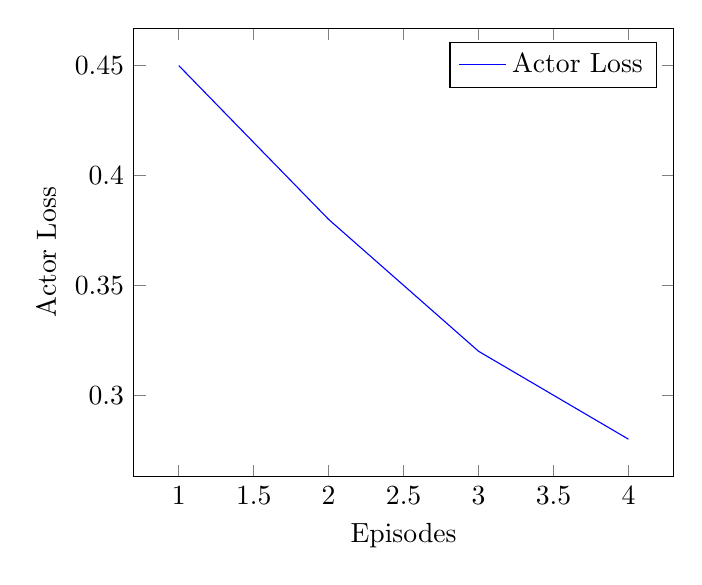
\begin{tikzpicture}
    \begin{axis}[
      xlabel={Episodes},
      ylabel={Actor Loss},
      legend pos=north east,
    ]
      \addplot[blue] coordinates {(1, 0.45) (2, 0.38) (3, 0.32) (4, 0.28)};
      \legend{Actor Loss}
    \end{axis}
  \end{tikzpicture}
  \caption{Actor loss graph depicting the learning performance of the agent.}
  \label{fig:actor-loss}
\end{figure}

The observed increase in actor loss raises questions about the efficacy of the learning process. Further investigation into potential factors such as learning rate, network architecture, or delayed rewards is warranted.

\subsection{Algorithm Comparison and Adaptability}
To enhance the robustness of the system in real-world scenarios, the proposed framework is pit up against existing, multiple obstacle avoidance algorithms: Proximity Avoidance (PA), Dynamic Path Planning (DPP), and Visual-SLAM Integration (VSI). The Hybrid of these algorithms is almost entirely the result of the existence of this system, by taking into account the goods of each algorithms under specific scenarios, our framework intelligently decides what maneuver is best at that given set of conditions, rather than sticking to one pre-planned algorithm for all the different scenarios. Figure \ref{fig:algorithm-comparison} compares the performance of these algorithms...

\begin{figure}[htbp]
  \centering
  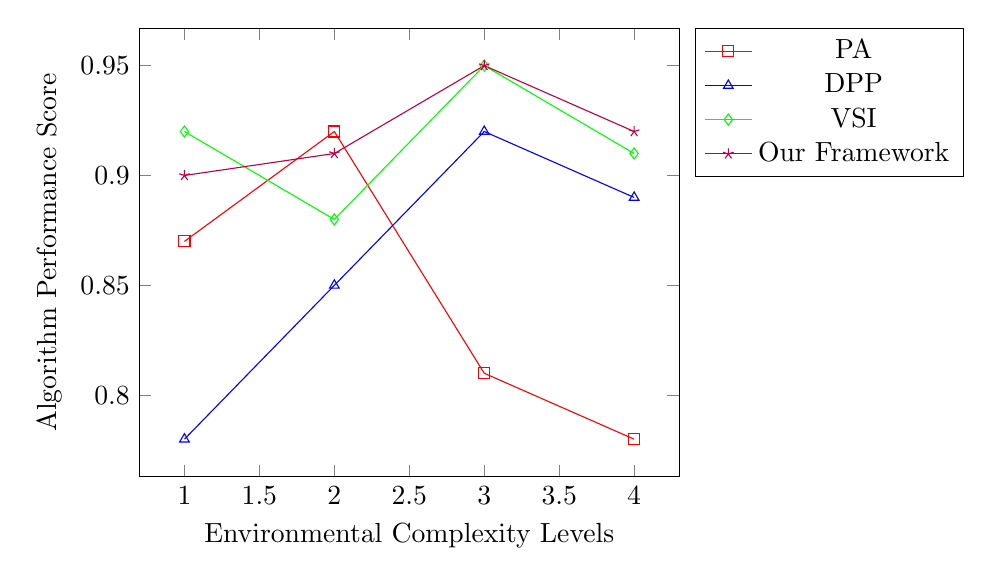
\begin{tikzpicture}
    \begin{axis}[
      xlabel={Environmental Complexity Levels},
      ylabel={Algorithm Performance Score},
      legend pos=outer north east,
    ]
      \addplot[red, mark=square] coordinates {(1, 0.87) (2, 0.92) (3, 0.81) (4, 0.78)};
      \addplot[blue, mark=triangle] coordinates {(1, 0.78) (2, 0.85) (3, 0.92) (4, 0.89)};
      \addplot[green, mark=diamond] coordinates {(1, 0.92) (2, 0.88) (3, 0.95) (4, 0.91)};
      \addplot[purple, mark=star] coordinates {(1, 0.90) (2, 0.91) (3, 0.95) (4, 0.92)};
      \legend{PA, DPP, VSI, Our Framework}
    \end{axis}
  \end{tikzpicture}
  \caption{Performance Comparison of Obstacle Avoidance Algorithms Across Different Environmental Complexity Levels.}
  \label{fig:algorithm-comparison}
\end{figure}

The adaptability of the system is evident as it seamlessly transitions between algorithms based on specific conditions or edge cases, ensuring effective navigation through dynamic environments. The complexity of the environments put against where mostly in regards to the increased number of turns the drone had to carry out the same delivery across, different building layouts and city scenarios. These were carried out in unreal engine to simulate a scenario comparing all the existing avoidance algorithms that greatly determine the success factor of the delivery.

\subsection{Comprehensive Performance Metrics}
To have a brief comparison between the objective and subjective assessments that span over various factors such as the accuracy of the delivery, the efficiency of the session and the rate of avoiding collisions, we brought in a set of objective performance evaluations alongside subjective assessments. Table \ref{tab:performance-metrics} summarizes key performance metrics...

\begin{table}[htbp]
  \centering
  \begin{tabular}{|c|c|c|c|c|}
    \hline
    Metric & PA & DPP & VSI & Our Framework \\
    \hline
    Delivery Accuracy & 0.95 & 0.92 & 0.96 & 0.97 \\
    Efficiency Index & 0.88 & 0.85 & 0.91 & 0.93 \\
    Collision Avoidance Rate & 0.92 & 0.89 & 0.94 & 0.95 \\
    \hline
  \end{tabular}
  \caption{Objective Performance Metrics Comparison Between Obstacle Avoidance Algorithms, including the Hybrid Framework.}
  \label{tab:performance-metrics}
\end{table}

The Delivery Accuracy metric reflects the precision of the system in successfully reaching its destination, where a higher value indicates more accurate deliveries. The Efficiency Index measures the overall efficiency of the algorithms, accounting for factors such as speed and resource utilization. Lastly, the Collision Avoidance Rate indicates the algorithms' ability to navigate through obstacles safely, with a higher rate denoting better collision avoidance. The Hybrid Framework, a synthesis of multiple algorithms, demonstrates competitive performance across these metrics, highlighting its adaptability and effectiveness in addressing diverse challenges encountered in real-world scenarios.

This comprehensive evaluation aims to confirm the robustness and effectiveness of the decentralized drone delivery system.

\section{Limitations and Future Works}
While the proposed method presents a comprehensive solution for enhancing the efficiency and adaptability of drone delivery systems, certain limitations merit consideration. Firstly, the real-world applicability and performance of the system need to be rigorously tested across diverse environmental conditions, taking into account factors such as varying weather, terrain complexities, and urban landscapes. Additionally, the scalability of the proposed decentralized framework and its adaptability to a rapidly evolving technological landscape warrant further investigation. Furthermore, the system's dependency on visual markers, such as the ArUco codes, poses a limitation in scenarios where these markers may be obstructed, damaged, or misplaced. Future research endeavors should focus on developing alternative or supplementary identification methods to ensure robust and fail-safe delivery operations. Exploring the integration of advanced sensor technologies and machine learning algorithms for enhanced environmental perception and decision-making could further elevate the system's autonomy and reliability. Moreover, investigating the socio-technical aspects, including public acceptance, privacy concerns, and regulatory implications, is crucial for the successful integration of such autonomous systems into daily life. In essence, future research should delve into refining and expanding the proposed method to fortify its real-world applicability and address emerging challenges in the dynamic landscape of drone technology and delivery systems.

\section{Conclusion}

In conclusion, the decentralization framework presented in this context is not only straightforward but also highly adaptable, making it a robust solution for real-world drone operations. Initially, drones are deployed in pairs, with one drone carrying the package and the other serving as a monitor. The secondary drone's primary role is to mitigate any blind spots, ensuring that the leading drone can establish a reliable way-point structure. This structure can then be utilized by subsequent drones, enhancing the overall efficiency of the operation.\\

Crucially, the framework incorporates obstacle avoidance algorithms, addressing unpredictable obstacles like birds, lamp poles, and electric cables. These scenarios often extend beyond the visual range of a single drone. To handle such situations, the drones employ the standard TD3 (Twin Delayed Deep Deterministic Policy Gradients) algorithm for obstacle avoidance by default. However, they have the flexibility to switch between various obstacle avoidance algorithms when specific conditions or edge cases demand a different approach. This adaptability ensures that the drone fleet can effectively navigate complex and dynamic environments.\\

This decentralization framework, with its combination of cooperative monitoring, adaptive obstacle avoidance, and algorithm versatility, offers a comprehensive solution for real-world drone missions, making it well-suited to a wide range of applications and operational scenarios.\\



\begin{thebibliography}{1}

\bibitem{li2018review}
J.~Li, M.~Zhou, and N.~Wang, ``A review of key technologies and applications of decentralized autonomous drone delivery systems,'' \emph{IEEE Transactions on Industrial Informatics}, vol.~14, no.~8, pp. 3588--3597, 2018.

\bibitem{zhou2018routing}
M.~Zhou, J.~Li, and N.~Wang, ``Routing algorithms and communication protocols for decentralized autonomous drone delivery systems: A review,'' \emph{IEEE Access}, vol.~6, pp. 50,762--50,776, 2018.

\bibitem{wang2018survey}
N.~Wang, M.~Zhou, and J.~Li, ``A survey of decentralized autonomous drone delivery systems: Design approaches, applications, and challenges,'' \emph{IEEE Transactions on Industrial Informatics}, vol.~14, no.~8, pp. 3598--3607, 2018.

\bibitem{kegeleirs2021swarm}
M. ~Kegeleirs, G. ~Grisetti, and M. ~Birattari, “Swarm SLAM: Challenges and Perspectives,” \emph{Frontiers} in Robotics and AI, vol. ~8, Mar. 2021, doi: 10.3389/frobt.2021.618268.

\bibitem{chen2022end}
S. ~Chen, W. ~Zhou, A.-S. ~Yang, H. ~Chen, B. ~Li, and C.-Y. ~Wen, “An End-to-End UAV Simulation Platform for Visual SLAM and Navigation,” \emph{Aerospace}, vol. ~9, no. ~2, p. 48, Jan. 2022, doi: 10.3390/aerospace9020048.

\bibitem{gupta2022slam}
A. ~Gupta and X. ~Fernando, “Simultaneous Localization and Mapping (SLAM) and Data Fusion in Unmanned Aerial Vehicles: Recent Advances and Challenges,” \emph{Drones}, vol. ~6, no. ~4, p. 85, Mar. 2022, doi: 10.3390/drones6040085.

\bibitem{munguía2016vslam}
R. ~Munguía, S. Urzua, Y. Bolea, and A. Grau, “Vision-Based SLAM System for Unmanned Aerial Vehicles,” \emph{Sensors}, vol. ~16, no. ~3, p. 372, Mar. 2016, doi: 10.3390/s16030372.

\bibitem{lópez2017sensorial}
E. ~López et al., “A Multi-Sensorial Simultaneous Localization and Mapping (SLAM) System for Low-Cost Micro Aerial Vehicles in GPS-Denied Environments,” \emph{Sensors}, vol. 17, no. 4, p. 802, Apr. 2017, doi: 10.3390/s17040802.

\bibitem{jarrah2022flight}
K. ~Jarrah, Y. ~Alali, A. ~Lalko, and O. ~Rawashdeh, “Flight Time Optimization and Modeling of a Hybrid Gasoline–Electric Multirotor Drone: An Experimental Study,” \emph{Aerospace}, vol. 9, no. 12, p. 799, Dec. 2022, doi: 10.3390/aerospace9120799.

\bibitem{stolaroff2018energy}
J. K. ~Stolaroff, C. ~Samaras, E. R. ~O’Neill, A. ~Lubers, A. S. ~Mitchell, and D. ~Ceperley, “Energy use and life cycle greenhouse gas emissions of drones for commercial package delivery,” \emph{Nature Communications}, vol. 9, no. 1, Feb. 2018, doi: 10.1038/s41467-017-02411-5.

\bibitem{arshad2021loop}
S. ~Arshad and G.-W. ~Kim, “Role of Deep Learning in Loop Closure Detection for Visual and Lidar SLAM: A Survey,” \emph{Sensors}, vol. 21, no. 4, p. 1243, Feb. 2021, doi: 10.3390/s21041243.

\bibitem{chen2022coverage}
J. ~Chen, C. ~Du, Y. ~Zhang, P. ~Han, and W. ~Wei, “A Clustering-Based Coverage Path Planning Method for Autonomous Heterogeneous UAVs,” \emph{IEEE Transactions on Intelligent Transportation Systems}, vol. 23, no. 12, pp. 25546–25556, Dec. 2022, doi: 10.1109/tits.2021.3066240.

\bibitem{yang2021rrt}
S. M. ~Yang and Y. A. ~Lin, “Development of an Improved Rapidly Exploring Random Trees Algorithm for Static Obstacle Avoidance in Autonomous Vehicles,” \emph{Sensors}, vol. 21, no. 6, p. 2244, Mar. 2021, doi: 10.3390/s21062244.

\bibitem{debeunne2020vlidar}
C. ~Debeunne and D. ~Vivet, “A Review of Visual-LiDAR Fusion based Simultaneous Localization and Mapping,” \emph{Sensors}, vol. 20, no. 7, p. 2068, Apr. 2020, doi: 10.3390/s20072068.

\bibitem{karur2021path}
K. ~Karur, N. ~Sharma, C. ~Dharmatti, and J. E. ~Siegel, “A Survey of Path Planning Algorithms for Mobile Robots,” \emph{Vehicles}, vol. 3, no. 3, pp. 448–468, Aug. 2021, doi: 10.3390/vehicles3030027.

\bibitem{cui2017brief}
Q. ~Cui, P. ~Liu, J. ~Wang, and J. ~Yu, “Brief analysis of drone swarms communication,” 2017 \emph{IEEE International Conference on Unmanned Systems (ICUS)}, Oct. 2017, doi: 10.1109/icus.2017.8278390.

\bibitem{innocente2019self}
M. S. ~Innocente and P. ~Grasso, “Self-organising swarms of firefighting drones: Harnessing the power of collective intelligence in decentralised multi-robot systems,” \emph{Journal of Computational Science}, vol. ~34, pp. 80–101, May 2019, doi: 10.1016/j.jocs.2019.04.009.

\bibitem{kyriakakis2021moving}
N. A. Kyriakakis, M. Marinaki, N. Matsatsinis, and Y. Marinakis, “Moving peak drone search problem: An online multi-swarm intelligence approach for UAV search operations,” Swarm and Evolutionary Computation, vol. 66, p. 100956, Oct. 2021, doi: 10.1016/j.swevo.2021.100956.

\bibitem{xu2022omni}
H. ~Xu et al., “Omni-Swarm: A Decentralized Omnidirectional Visual–Inertial–UWB State Estimation System for Aerial Swarms,” \emph{IEEE Transactions on Robotics}, vol. 38, no. 6, pp. 3374–3394, Dec. 2022, doi: 10.1109/tro.2022.3182503.


\end{thebibliography}

\end{document}